\documentclass[11pt]{article}
%%%%%%%%%%%%%%%%
% Packages
%%%%%%%%%%%%%%%%

\usepackage[top=1cm,bottom=1cm,left=1.5cm,right= 1.5cm]{geometry}
\usepackage[parfill]{parskip}
\usepackage{graphicx, fontspec, xcolor, multicol, enumitem, setspace}
\DeclareGraphicsRule{.tif}{png}{.png}{`convert #1 `dirname #1`/`basename #1 .tif`.png}

%%%%%%%%%%%%%%%%
% Sakai link - update each semester
%%%%%%%%%%%%%%%%

\newcommand{\Sakai}[1]
{\href{https://sakai.duke.edu/portal/site/ef372254-413e-42f6-b414-f8bc91a58fa0/page/98390abf-b461-44cb-a062-aa6864748ab3}{Sakai}}


%%%%%%%%%%%%%%%%
% No page number
%%%%%%%%%%%%%%%%

\pagestyle{empty}

%%%%%%%%%%%%%%%%
% User defined colors
%%%%%%%%%%%%%%%%

% Pantone 2015 Spring colors
% http://iwork3.us/2014/09/16/pantone-2015-spring-fashion-report/
% update each semester or year

\xdefinecolor{custom_blue}{rgb}{0, 0.70, 0.79} % scuba blue
\xdefinecolor{custom_darkBlue}{rgb}{0.11, 0.31, 0.54} % classic blue
\xdefinecolor{custom_orange}{rgb}{0.97, 0.57, 0.34} % tangerine
\xdefinecolor{custom_green}{rgb}{0.49, 0.81, 0.71} % lucite green
\xdefinecolor{custom_red}{rgb}{0.58, 0.32, 0.32} % marsala

\xdefinecolor{custom_lightGray}{rgb}{0.78, 0.80, 0.80} % glacier gray
\xdefinecolor{custom_darkGray}{rgb}{0.54, 0.52, 0.53} % titanium

%%%%%%%%%%%%%%%%
% Color text commands
%%%%%%%%%%%%%%%%

%orange
\newcommand{\orange}[1]{\textit{\textcolor{custom_orange}{#1}}}

% yellow
\newcommand{\yellow}[1]{\textit{\textcolor{yellow}{#1}}}

% blue
\newcommand{\blue}[1]{\textit{\textcolor{blue}{#1}}}

% green
\newcommand{\green}[1]{\textit{\textcolor{custom_green}{#1}}}

% red
\newcommand{\red}[1]{\textit{\textcolor{custom_red}{#1}}}

%%%%%%%%%%%%%%%%
% Coloring titles, links, etc.
%%%%%%%%%%%%%%%%

\usepackage{titlesec}
\titleformat{\section}
{\color{custom_blue}\normalfont\Large\bfseries}
{\color{custom_blue}\thesection}{1em}{}
\titleformat{\subsection}
{\color{custom_blue}\normalfont}
{\color{custom_blue}\thesubsection}{1em}{}

\newcommand{\ttl}[1]{ \textsc{{\LARGE \textbf{{\color{custom_blue} #1} } }}}

\newcommand{\tl}[1]{ \textsc{{\large \textbf{{\color{custom_blue} #1} } }}}

\usepackage[colorlinks=false,pdfborder={0 0 0},urlcolor= custom_orange,colorlinks=true,linkcolor= custom_orange, citecolor= custom_orange,backref=true]{hyperref}

%%%%%%%%%%%%%%%%
% Instructions box
%%%%%%%%%%%%%%%%

\newcommand{\inst}[1]{
\colorbox{custom_blue!20!white!50}{\parbox{\textwidth}{
	\vskip10pt
	\leftskip10pt \rightskip10pt
	#1
	\vskip10pt
}}
\vskip10pt
}

%%%%%%%%%%%%%%%%
% Timing
%%%%%%%%%%%%%%%%

% 12-15 minutes

%%%%%%%%%%%%%%%%
% Sakai link for course
%%%%%%%%%%%%%%%%

% UPDATE FOR OWN COURSE
% LINK TO ASSIGNMENTS TOOL IN SAKAI

\newcommand{\Sakai}[1]
{\href{https://sakai.duke.edu/portal/site/ba0d1c18-ba55-473f-9d70-b6a1f9559bbe/page/9870858b-a1a9-481e-8497-8a6ffe9e5be2}{Sakai}}

%%%%%%%%%%%
% App Ex number    %
%%%%%%%%%%%

% DON'T FORGET TO UPDATE

\newcommand{\appno}[1]
{3.2}

%%%%%%%%%%%%%%
% Turn on/off solutions       %
%%%%%%%%%%%%%%

% Off
\newcommand{\soln}[1]{
\vskip5pt
}

%% On
%\newcommand{\soln}[1]{
%\textit{\textcolor{custom_darkGray}{#1}}
%}

%%%%%%%%%%%%%%%%
% Document
%%%%%%%%%%%%%%%%

\begin{document}
\fontspec[Ligatures=TeX]{Helvetica Neue Light}

Dr. \c{C}etinkaya-Rundel \hfill Data Analysis and Statistical Inference \\

\ttl{Application exercise \appno{}: \\
Hypothesis testing for a single mean}

\inst{Submit your responses on \Sakai{}, under the appropriate assignment. Only one submission per team is required. One team will be randomly selected and their responses will be discussed.}

%%%%%%%%%%%%%%%%%%%%%%%%%%%%%%%%%%%%


In 2001 the average GPA of students at Duke University was 3.37. Last semester 63 Sta 101 students responded to the question on GPA on the class survey. The mean was 3.58, and the standard deviation 0.53. A histogram of the data is shown below.

\begin{center}
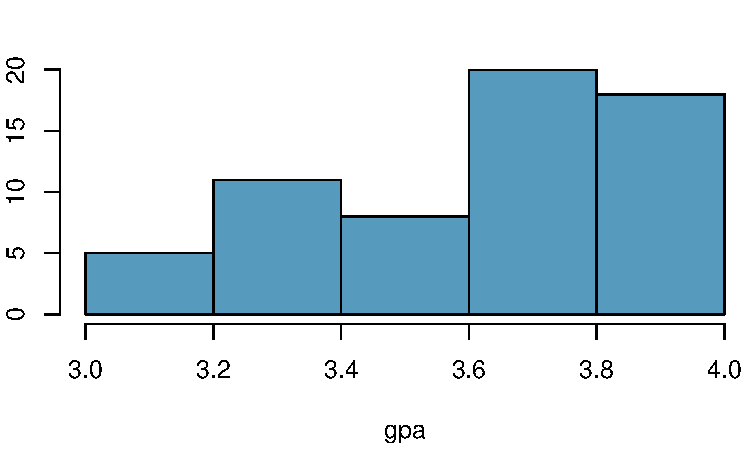
\includegraphics[width=0.5\textwidth]{survey/hist_gpa}
\end{center}

Assuming that this sample is random and representative of all Duke students (bit of a leap of faith? you can discuss that when checking the conditions), do these data provide convincing evidence that the average GPA of Duke students has \textbf{\underline{changed}} over the last decade and a half?

Make sure to check conditions, note any assumptions you make, and show all your work.

%> Z = (3.58-3.37)/(.53/sqrt(63))
%> pnorm(Z, lower.tail = FALSE)*2
%[1] 0.0016

%%%%%%%%%%%%%%%%%%%%%%%%%%%%%%%%%%%%

\end{document}